\label{sec:evaluation}

We perform all of our evaluations on a quiescent 8-core system (dual processor with 4 cores), with 8GB of RAM. Each processor is a 4-core 64-bit Intel Xeon, running at 2.33 Ghz with a 4MB L2 cache. For compatibility reasons, we compile all applications to a 32-bit target using the GCC compiler. All performance data is the average of ten runs, excluding the maximum and minimum values.

The evaluation answers the following questions:

\begin{itemize}
\item How effective is \sheriffdetect{} at finding false sharing and guiding programmers to their resolution? (Section~\ref{sec:effecteval})
\item What is \sheriffdetect{}'s performance overhead? (Section~\ref{sec:results-runtime-overhead})
\item How sensitive is \sheriffdetect{} to different sampling rate? (Section~\ref{sec:results-sampling-overhead}) 
\item How effective does \sheriffprotect{} mitigate false sharing? (Section~\ref{sec:protectperformance})
\end{itemize}

\subsection{\sheriffdetect{} Effectiveness}

\label{sec:effecteval}

This section evaluates whether \sheriffdetect{} can be used to find false sharing problems, both in synthetic test cases and in actual applications.

We developed a range of microbenchmarks that exemplify different situations related to false sharing. We evaluate these benchmarks on both \SheriffDetect{} and Intel's Performance Tuning Utility(PTU v3.2), the previous state-of-the-art work of false sharing detection. 

Detection results are shown in Table~\ref{table:microbenchmarks}. \sheriffdetect{} only reports those false sharing instances that can possibly affect the performance, while correctly ignores those cases without performance impact.
PTU has false alarms/positives.  It does not track access patterns, which reports false positives for those non-interleaved accesses. Also, PTU does not track memory deallocations, thus it can not filter out those pseudo false sharing caused by memory reuse. \sheriffdetect{} avoids all of these problems and reports false sharing problems correctly. 


\begin{table}
\centering
\resizebox{\columnwidth}{!}{
\begin{tabular}{l|l|l|l}
\hline
{\bf \small Microbenchmark} & {\bf \small Perf Sensitive } & {\bf \small \sheriffdetect{} } & {\bf \small PTU } \\
\hline

\small \textbf{False Sharing (adjacent objects)} & YES & \cmark{} & \cmark{} \\
\small \textbf{False Sharing (same object)} & YES & \cmark{} & \cmark{} \\
\hline
\small \textbf{True Sharing} & NO & & \\
\small \textbf{Non-interleaved False Sharing} & NO & & \xmark{}\\
\small \textbf{Heap Reuse(no sharing)} & NO & & \xmark{}\\
\hline
\end{tabular}
}
\caption{False sharing detection results using PTU and \sheriffdetect{}. \sheriffdetect{} correctly reports only actual false sharing instances that have performance impact;
\cmark{} indicates a correct report and \xmark{} indicates a false alarm. 
\label{table:microbenchmarks}}
\end{table}

We further evaluate \SheriffDetect{} and PTU on two widely-used benchmark suites, Phoenix~\cite{phoenix-hpca} and PARSEC~\cite{parsec}. We use the simlarge inputs for all applications of PARSEC. For Phoenix, we chose available parameters that allow the programs to run as long as possible. As of this writing, we were unable to successfully compile \texttt{raytrace} and \texttt{vips}, and \sheriff{} is
currently unable to run \texttt{x264}, \texttt{bodytrack},
and \texttt{facesim}. \texttt{Freqmine} currently can not support \pthreads{}. Thus, those benchmarks are excluded here. 
 
\begin{table}
\centering
\begin{tabular}{l|r|r}
\hline
{\bf \small Benchmark} & {\bf \small PTU} & {\bf \small \sheriffdetect{}}\\
 & {\# Lines} & {\# Objects}\\
\hline
\small \textbf{kmeans} & 1916 &  2 \\
\small \textbf{linear\_regression} & 5 & 1 \\
\small \textbf{matrix\_multiply} & 468 & 0\\
\small \textbf{pca} & 45 & 0 \\
\small \textbf{reverseindex} & N/A & 5 \\
\small \textbf{word\_count} & 4 & 3\\
\hline
\small \textbf{canneal} & 1 & 1 \\
\small \textbf{fluidanimate} & 3 & 1 \\
\small \textbf{streamcluster} & 9 & 1\\
\small \textbf{swaptions} & 196 & 0\\
\hline
\small \textbf{Total} & 2647 & 14\\
\hline
\end{tabular}
\caption{Overall detection results of PTU and \sheriffdetect{} on Phoenix and PARSEC benchmark suites. We only list those benchmarks that at least one of tools reports false sharing problems. For PTU, we show how many cache lines are marked as falsely shared. For \sheriffdetect{}, we show how many objects are reported by \sheriffdetect{} (with cache invalidations larger than 100). The item marked as ``N/A'' means that PTU fails to show results because it runs out of memory.
\label{table:fsdetection}}
\end{table}


The overall results are shown in Table~\ref{table:fsdetection}. PTU reports that 2647 cache lines may exist false sharing problems, given that they can report false positives. \sheriffdetect{} reveals that seven out of sixteen evaluated benchmarks have false sharing problems. Totally, only 14 objects are reported, but only 4 of them shows a big number of cache invalidations, thus needs to be fixed. 

Several reasons contributes to the number difference between these two approaches. First, PTU reports cache lines involving in false sharing, while \SheriffDetect{} only reports objects. If an object has a size larger than the size of cache line, PTU can report multiple times, one on each cache line. Second, PTU reports multiple times if a heap object, with the same allocation site, is allocated multiple times, while \SheriffDetect{} only reports once. Third, PTU may report false positives since it do not track interleaved accesses and overrate the problems caused by heap reuses. 

We manually fix these four false sharing problems based on reports of \SheriffDetect{}, and show the performance gains after fixes in Table~\ref{table:perfafterfix}. To explain why performance improvement are different, we also examine the maximum possible updates that can occur on a false sharing object, although the actual number of interleaved accesses depends on scheduling. For example, \texttt{linear\_regression} has the largest updates, thus causing the most serious performance problem. 

\begin{table}
\centering
\begin{tabular}{l|r|r}
\hline
{\bf \small Benchmark} & {\bf \small Performance Improvement} & {\bf \small Updates}\\
 & & (M)\\
\hline
\small \textbf{linear\_regression} & 818\% & 1323.6\\
\small \textbf{reverseindex} &  2.4\% & 0.4\\
\small \textbf{streamcluster} & 5.4\% & 28.7\\
\small \textbf{word\_count} &  1\% & 0.3\\
\hline
\end{tabular}
\caption{Performance data for four false sharing benchmarks. All data are obtained using the standard \pthreads{} library. ``Updates'' shows how many million updates (in total) occurred on falsely-shared cache lines.
\label{table:perfafterfix}}
\end{table}


In \texttt{reverse\_index} and \texttt{word\_count}, multiple threads repeatedly modify the same heap object. The pseudo code for these two benchmarks are listed in Figure~\ref{fig:reverseindex}. For these two benchmarks, we can use thread-local variables to avoid performance problems: each thread can operate on a temporary variable first, and then modify the global \texttt{use\_len} at the end of the thread.

\begin{figure}[!t]
\begin{lstlisting}[style=tt]
int * use_len;
void insert_sorted(int curr_thread) {
   ......	
   // After finding a new link
   (use_len[curr_thread])++;
   ......	
}
\end{lstlisting}
\caption{A fragment of source code from \texttt{reverse\_index}. False sharing arises when different threads 
modify different words in the same \texttt{use\_len} array. 
\label{fig:reverseindex}}
\end{figure}

\texttt{Linear\_regression}'s false sharing problem is a little different (see Figure~\ref{fig:linear_regression}). 
Two different threads write to the same cache line when the structure \texttt{lreg\_args} is not aligned with corresponding cache lines. This problem can be avoided easily by padding the structure \texttt{lreg\_args}, thus preventing different threads concurrently accessing the same cache line. 

\begin{figure}[!t]
\begin{lstlisting}[style=tt]
struct {
  long long SX;
  long long SY;
  long long SXX;
  ......
} lreg_args;

void *lreg_thread(void *args_in) {
  struct lreg_args * args = args_in;
  for(i = 0; i < args->num_elems; i++) {
    args->SX  += args->points[i].x;
    args->SXX += args->points[i].x 
   	         * args->points[i].x;
  }
  ......	
}
\end{lstlisting}
\caption{A fragment from \texttt{linear\_regression} code. Each thread is passed in a different address (\texttt{struct lreg\_args}) and each thread can work on its corresponding \texttt{args\_in}. 
Unfortunately, the size of \texttt{struct lreg\_args} is not cache line aligned (52 bytes) on 32-bit machine and that causes two different threads to write to the same cache line simultaneously. 
\label{fig:linear_regression}}
\end{figure}

The false sharing problem detected in \texttt{streamcluster} (one of the PARSEC benchmarks) is similar to that in \texttt{linear\_regression}: two different threads are writing to the same cache line. Examination of the source code indicates that the author tried to avoid false sharing by padding, but the amount of padding, 32 bytes, was insufficient to accommodate the actual physical cache line size used in the evaluation (64 bytes). Setting the \texttt{CACHE\_LINE} macro to 64 bytes avoids this false sharing problem.


\subsubsection{Ease of locating false sharing problems}

\label{sec:fsfixexample}

To illustrate how \sheriffdetect{} can precisely locate false sharing problems, we use one benchmark (\texttt{word\_count}, a Phoenix benchmark) as an example. Our experience with diagnosing other false sharing issues is similar.

Here is an example output from \sheriffdetect{} for \texttt{word\_count}.

\begin{verbatim} 
1st object, cache interleaving writes 
13767 times (start at 0xd5c8e140). 
Object start 0xd5c8e160, length 32. 
It is a heap object with callsite:
[0]: ./wordcount_pthreads.c:136
[1]: ./wordcount_pthreads.c:441
\end{verbatim}

Line 136 (\texttt{wordcount\_\pthreads{}.c}) contains the following memory allocation:

\begin{verbatim}
use_len=malloc(num_procs*sizeof(int));
\end{verbatim}

Grepping for \texttt{use\_len}, a global pointer, quickly leads to this line:

\begin{verbatim}
use_len[thread_num]++;
\end{verbatim}

Now it is clear that different threads are modifying the same object(use\_len). Fixing the problem by using a thread-local data copy is now straightforward.

By contrast, we can compare PTU's output that shown in Figure~\ref{fig:wordcount}. Finding this problem is far more complicated with PTU. PTU only presents functions using each cache line, not to mention the fact that PTU can report huge numbers of false positives.  Another shortcoming of PTU is that ``Collected Data Refs'' number cannot be used as a metric to evaluate the significance of false sharing problems. For this example, PTU only reports 12 references, while \sheriffdetect{} observes 13767 cache invalidations.

\begin{figure*}[!t]
\centering
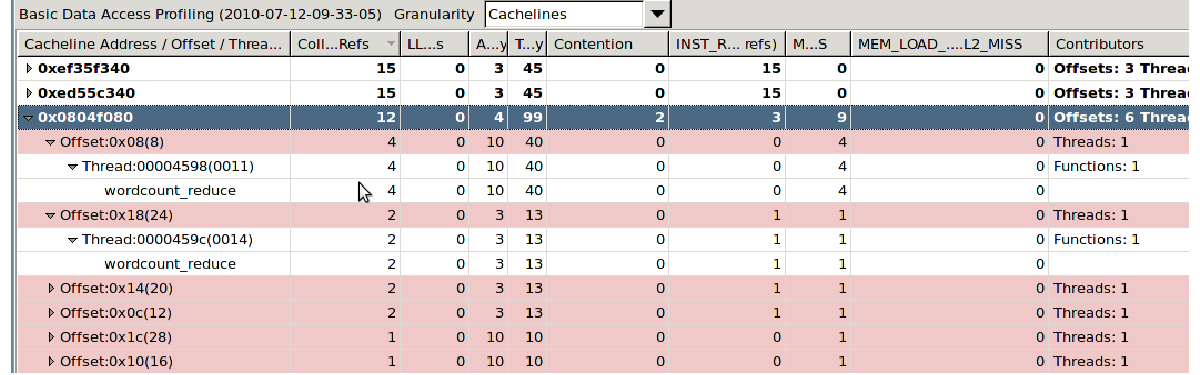
\includegraphics[width=6in]{sheriff/figure/wordcount}
\caption{PTU output for \texttt{word\_count}.
\label{fig:wordcount}}
\end{figure*}

\subsection{\sheriffdetect{} Performance Overhead}
\label{sec:results-runtime-overhead}

\begin{figure*}[!t]
\centering
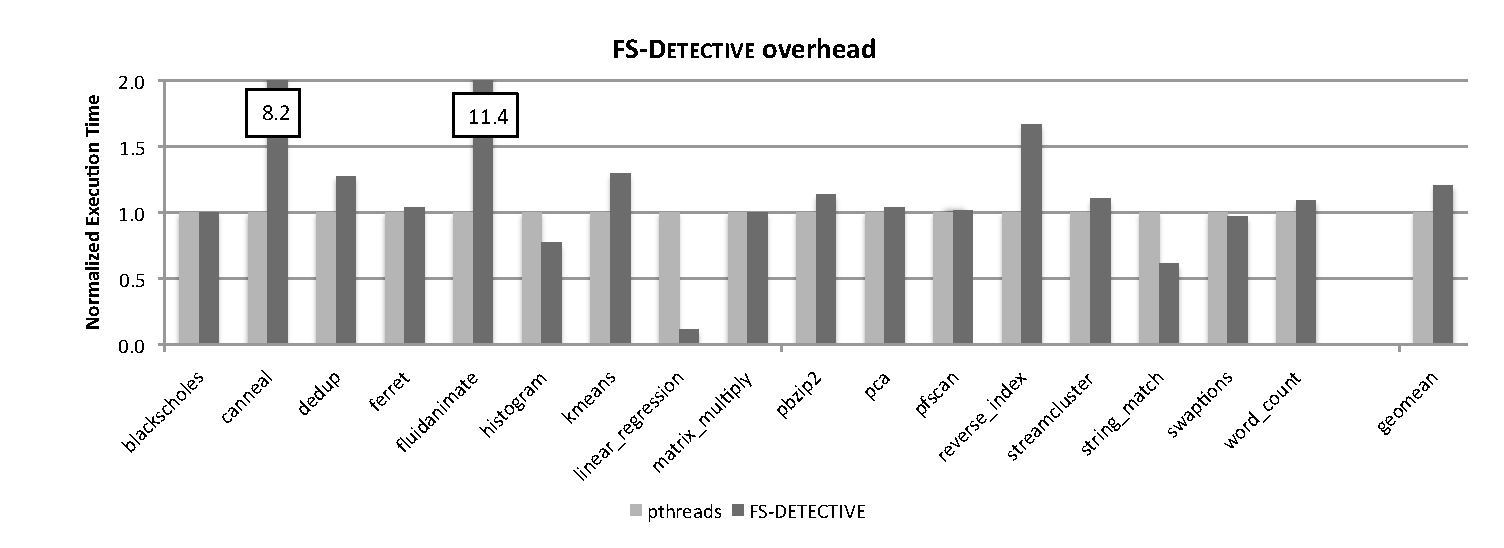
\includegraphics[width=6in]{sheriff/figure/detectiveperf.pdf}
\caption{\sheriffdetect{} performance overhead across two suites of benchmarks, normalized to the runtime of using the \pthreads{} library (lower is better). \label{fig:overhead}}
\end{figure*}


\SheriffDetect{}'s  runtime overhead (comparing to \pthreads{}) on two multithreaded benchmarks suites, Phoenix and PARSEC is shown in Figure~\ref{fig:overhead}.  \SheriffDetect{} only introduces 20\% performance on average, with the exception of three outliers. For other benchmarks, \SheriffDetect{}’s overhead is generally acceptable and far lower than most previous tools.


There are two benchmarks on which \sheriffdetect{} do not perform well. \texttt{canneal} runs about $7\times$ slower than that with \pthreads{}.  \texttt{fluidanimate}'s  performance overhead is about $11\times$ slower than that using \pthreads{}.

The first reason for these overheads is that both benchmarks
trigger a high number of dirtied pages (3.4 million and
2.15 million, respectively). For each dirty page, \sheriffdetect{} applies page protection twice, create a ``copy-on-write'' page and a ``twin'' page, checks false sharing problems at every sampling interval, and commits those local changes to the shared mapping. Thus, given large amount of dirty pages, copying overhead alone is very expensive and can dominate most of overhead. For example, \texttt{Canneal} invokes around 3.4 million dirty pages, thus leading to substantial overhead. 

\texttt{fluidanimate} also runs slowly with \SheriffDetect{}
because of an unusually high number of transactions (16.7
million). Since \SheriffDetect{} replaces lock calls with their interprocess variants and triggers a transaction end and begin for each lock calls, thus, adding overhead if there are shared pages.
 
 
While these outliers force \SheriffDetect{} to run
slowly, \SheriffDetect{}’s overhead is generally acceptable
and far lower than most previous tools.

\texttt{linear\_regression} is an outlier in the opposite direction: with \SheriffDetect{}, it runs $8\times$ faster than with \pthreads{}, even with the added overhead of protection, memory commits, sampling and 
other mechanisms.  There is a serious false sharing problem inside (see Table~\ref{table:perfafterfix},) which both \sheriffdetect{} and \sheriffprotect{} eliminate automatically. Other cases where \sheriffdetect{}
outperforms \pthreads{} are also due to false sharing elimination;
\SheriffProtect{} further reduces overhead for these
and other applications, as the next section describes.

%%%%%%%%%%%%%%%%%%%%%%%%%%%%%%%%%%%%%%%5
%%%% Some data to list the effectiveness of this tool.
%%%%%% How many caches are carried for each test case. 
%%%%%% Whether all caches has false sharing problem.
%%%%%%%%%%%%%%%%%%%%%%%%%%%%%%%%%%%%%%%
\subsection{\SheriffDetect{} Sampling Rate Sensitivity}
\label{sec:results-sampling-overhead}

\SheriffDetect{} employs the sampling mechanism to detect false sharing happening in long-running transactions. Sampling is only triggered when the length of a transaction exceeds a pre-defined threshold, usually 10ms. By handling those \texttt{SIGALARM} signals, \SheriffDetect{} tracks memory accesses by by comparing the temporary twin page against its
corresponding working version, and updates status words of specific cache lines. Thus, increased sampling rates may uncover more false sharing problems, but at the cost of increase performance overhead. 

To measure \sheriffdetect{}'s sensitivity to the sampling rate, we evaluate on three different sampling rates: 2ms, 10ms (our baseline), and 50ms.

\paragraph{Sampling Overhead:} Figure~\ref{fig:sensitivity} shows the performance overhead under these different sampling rates, normalized to the runtime of using  the default 10ms sample rate. For most of these benchmarks, sampling imposes relatively little overhead because the average
number of shared pages is not large or because the
transaction length is often shorter than the sampling interval.

One outlier is \texttt{canneal}, which is extremely sensitive to the sampling rate.  When the sampling interval is 2ms, \texttt{canneal} runs about $2.3\times$ slower than that with  a 10ms sampling interval; \texttt{canneal} runs 35\% slower with a 50ms sampling interval than 2 10ms
sampling interval. The reason is that \texttt{canneal} dirties a large number of shared pages. More frequent sampling thus increases the amount of checking overhead.


\begin{figure*}[!t]
\centering
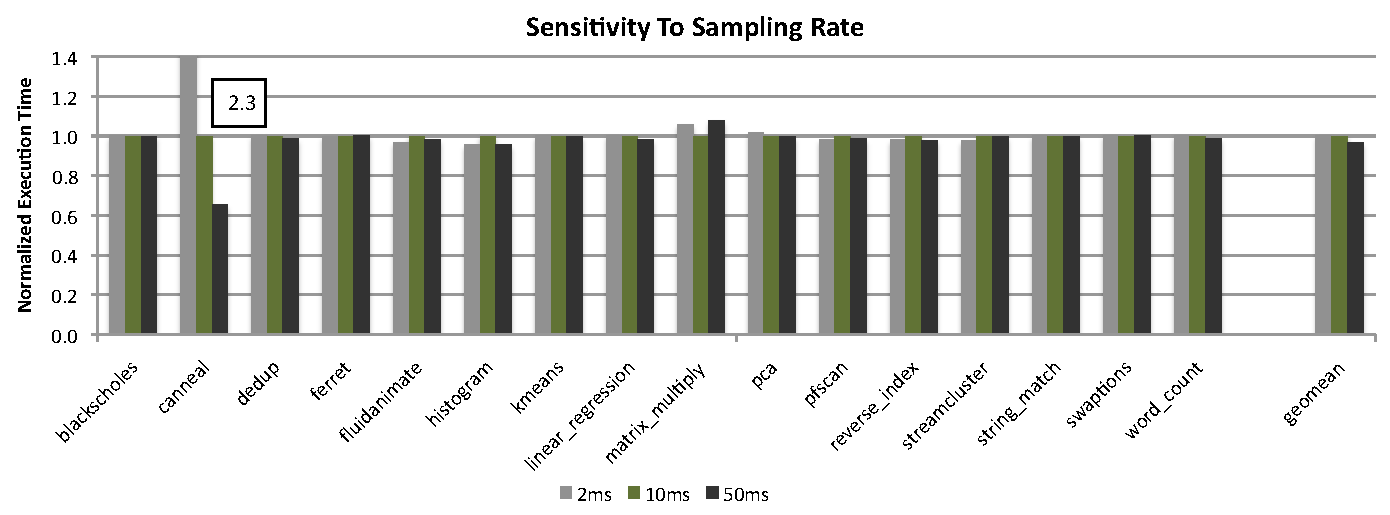
\includegraphics[width=5in]{sheriff/figure/sensitivity}
\caption{\sheriffdetect{} performance with different sampling rates,  normalized to the performance with a sampling interval of 10ms (presented in Figure~\ref{fig:overhead}); lower is better.
\label{fig:sensitivity}}
\end{figure*}

\begin{table*}[!t]
\centering
\resizebox{\columnwidth}{!}{
\begin{tabular}{l|rr|rr|rr}
\hline
{\bf \small Benchmark} & \multicolumn{2}{c|} {\bf \small 2ms} & \multicolumn{2}{c|} {\bf \small 10ms}& \multicolumn{2}{c} {\bf \small 50ms}\\
& {\em objs}  & {\em writes} & {\em objs}  & {\em writes} & {\em objs}  & {\em writes} \\
\hline
\small \texttt{canneal} & 1 & 21444321 & 1 & 26369324 & 1 & 30580451 \\
\small \texttt{ferret} & 1 & 3 & 0 & 0 & 0 & 0 \\
\small \texttt{fluidanimate} & 1 & 3370 & 1 & 4064 & 1 & 2851 \\
\small \texttt{kmeans} & 2 & 2974 & 2 & 1122 & 1 & 98 \\
\small \texttt{linear\_regression} & 1 & 1050 & 1 & 311 & 1 & 71 \\
\small \texttt{reverse\_index} & 5 & 14494 & 5 & 14782 & 5 & 14981 \\
\small \texttt{streamcluster} & 2 & 52462 & 1 & 52283 & 1 & 52420 \\
\small \texttt{word\_count} & 4 & 9849 & 4 & 2699 & 3 & 622 \\
\hline
\end{tabular}
}
\caption{
\sheriffdetect{} precision with different sampling rates, including the number of falsely-shared objects and interleaved writes. We omit those benchmarks with no observed cases of false sharing.
\label{table:samplingquality}}
\end{table*}

\paragraph{Sampling Effectiveness:}
The choice of sampling rates has relatively little impact on detection and ranking, shown in Table~\ref{table:samplingquality}. As anticipated, in most cases, the number of falsely-shared objects reported and the number of interleaved writes observed are not significantly different.

Changing the sampling rate can affect the number of falsely-shared objects detected, but \SheriffDetect{} reports all instances with a significant performance impact under the default sampling rate. Increasing the sampling rate to 2ms reveals two additional falsely-shared objects (for \texttt{ferret} and \texttt{streamcluster}), but the number of additional interleavings is quite low (under 10 for those objects). Similarly, reducing the sampling rate to 50ms results in the detection of two fewer objects overall (\texttt{kmeans} and \texttt{word\_count}), but these objects have little impact on performance.


\subsection{\SheriffProtect{} Performance Overhead}
\label{sec:protectperformance}

\begin{figure*}[!t]
\centering
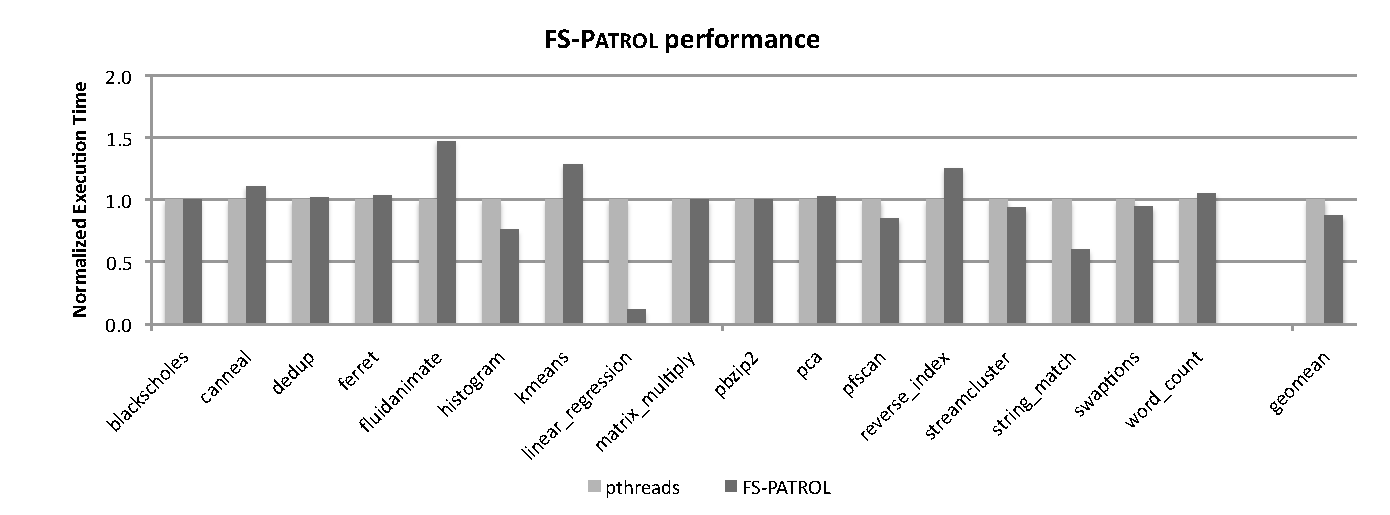
\includegraphics[width=5in]{sheriff/figure/patrolperf.pdf}
\caption{\sheriffprotect{} performance across two suites of benchmarks, normalized to the performance of the \pthreads{} library (see Section~\ref{sec:results-runtime-overhead}). In case of catastrophic false sharing, \sheriffdetect{} dramatically increases performance.
\label{fig:patrol}}
\end{figure*}

\begin{table}[!t]
\centering
\begin{tabular}{l|r|r}
\hline
{\bf \small Benchmark} & \multicolumn{2}{c} {\bf \small Normalized Runtime} \\
% \cline{2-3}
 & {\bf \small \sheriffdetect{} }  & {\bf \small \sheriffprotect{}} \\
\hline
\small \texttt{blackscholes} & 1.00 & 1.00 \\
\small \texttt{canneal} &  8.23 & 1.11 \\
\small \texttt{dedup} & 1.27 & 1.02 \\
\small \texttt{ferret} & 1.03 & 1.03\\
\small \texttt{fluidanimate} & 11.39 & 1.47 \\
\small \texttt{histogram} & \textbf{0.77} & \textbf{0.76} \\\small \texttt{kmeans} & 1.29 & 1.28 \\
\small \texttt{linear\_regression} & \textbf{0.12} & \textbf{0.11} \\
\small \texttt{matrix\_multiply} & 1.00 & 1.00 \\
\small \texttt{pbzip2} & 1.13 & 1.00 \\
\small \texttt{pca} & 1.04 & 1.03 \\
\small \texttt{pfscan} & 1.02 & \textbf{0.85} \\
\small \texttt{reverse\_index} & 1.67 & 1.25 \\
\small \texttt{streamcluster} & 1.10 &  \textbf{0.94} \\
\small \texttt{string\_match} & \textbf{0.61} & \textbf{0.60} \\
\small \texttt{swaptions} & \textbf{0.97} & \textbf{0.94} \\
\small \texttt{word\_count} & 1.09 & 1.05\\
\hline
\small \textbf{\em Geomean} & 1.21 & \textbf{0.87} \\
\hline
\end{tabular}
\caption{Detailed execution times with \sheriffdetect{} and \sheriffprotect{}, normalized to execution with the \pthreads{} library; numbers below 1 (boldfaced) indicate a speedup over \pthreads{}.
\label{table:detailedperf}}
\end{table}

Here, we examine the effectiveness of eliminating false sharing problems.  Figure~\ref{fig:patrol} presents the performance under \SheriffProtect{} and the standard \pthreads{} library.  For most cases, \SheriffProtect{} either has no effect on performance (when there is no false sharing problem inside) or improves the performance. Table~\ref{table:detailedperf} presents detailed performance results of \SheriffDetect{} and \SheriffProtect{}. 

\SheriffProtect{} improves the performance when an application is detected to have false sharing problems inside.  \texttt{linear\_regression} exhibits almost a $10\times$ speedup against the one using \pthreads{} library, by tolerating a serious false sharing problem inside (see Table~\ref{table:perfafterfix}). \texttt{histogram} runs substantially faster with \SheriffProtect{} (24\%), although we currently are not certain why this is the case. \texttt{string\_match} runs 40\% faster because of false sharing caused by the \pthreads{} heap allocator, which is why \SheriffDetect{} does not find. 

There are three benchmarks which runs up to 47\% slower than using the \pthreads{}. 
\texttt{kmeans} creates more than 3000 threads in eight seconds. Since the overhead of creating one process is higher than that of creating one thread, this dominates most of overhead. 

For \texttt{reverse\_index} and \texttt{fluidanimate}, 
they exhibit slowdown because of using the processes-as-threads framework. The \Sheriff{} framework connects the private mapping and shared mapping using of a file-based mapping, operating on those file-based pages is more expensive than operating on anonymous pages (the normal status of heap-allocated pages) under the Linux. For example, the shared store for all heap pages is initially set to \texttt{MAP\_SHARED}, so writing to one shared page can cause a Copy-On-Write operation in the kernel even when there is only one user. 

\texttt{fluidanimate} has an enormous number of transactions(18 Million), \sheriffprotect{} 
introduces some additional overhead for every transaction. That also accounts for part of overhead.
